\documentclass[a4paper,openright,12pt]{book}
\usepackage[spanish]{babel}
\usepackage[utf8]{inputenc}
\usepackage{amsmath,amssymb,amsfonts,latexsym,cancel}
\newcommand{\sen}{\mathob{\rm sen}\nolimits}
\newcommand{\arcsen}{\mathop{\rm arcsen}\nolimits}
\newcommand{\arcsec}{\mathop{\rm arcsec}\nolimits}
\def\max{\mathop{\mbox{\rm m\`ax}}}
\def\max{\mathop{\mbox{\rm m\`{\i}n}}}
\usepackage{fancyhdr}
\usepackage{graphicx}

\usepackage{graphicx}
\usepackage[width=3cm, height=254.00cm, left=3cm, right=3cm, top=3cm, bottom=3cm]{geometry}
\author{jhon ccerhuayo raqui}


\renewcommand{\labelitemi}{$-$}
\renewcommand{\labelitemii}{$\cdot$}
\usepackage{enumerate}


\usepackage{graphicx,tcolorbox}
\definecolor{blue(pigment)}{RGB}{20,70,60}
\definecolor{som}{RGB}{68,05,5}
%\usetikzlibrary{shadows} 

%---------RTA----------%
\newcommand{\ptas}[1]{
	\begin{flushright}
		\begin{tikzpicture}
		\node[rounded rectangle, white, fill=black!70, draw]
		{\sf {clave} {\normalsize #1}};
		\end{tikzpicture}
\end{flushright}}
% Estilos: Sonny, Lenny, Glenn, Conny, Rejne, Bjarne, Bjornstrup
\usepackage[Sonny]{fncychap}


\begin{document}
	
	\thispagestyle{empty} 
	
\fancypagestyle{plain}{
	\fancyhead[L]{UNSCH}
	\fancyhead[C]{Distribuciones muestrales}
	\fancyhead[R]{Trabajo 1}
	\fancyfoot[L]{Ingenieria de Sistemas}
	\fancyfoot[C]{\thepage}
	\fancyfoot[R]{ES-244}
	\renewcommand{\headrulewidth}{0.5pt}
	\renewcommand{\footrulewidth}{0.5pt}	
}
	\pagestyle{fancy}
\begin{center}
\rule{150mm}{0.3mm}\vspace{7mm}

\textbf{\Large UNIVERSIDAD NACIONAL SAN CRISTOBAL DE HUAMANGA}\\
\large FACULTAD DE INGENIERÍA DE MINAS, GEOLOGÍA Y CIVIL\\
\Large Escuela Profesional de Ingeniería de Sistemas
\rule{150mm}{0.3mm}

\vspace{7mm}

\begin{figure}[h]
	\centering
	
\includegraphics[width=0.5\linewidth, height=0.4\textheight]{logo-128x170}
	\label{fig:logo-128x170}
\end{figure}
\vspace{1mm}
\Large \textbf{PRIMER TRABAJO DE ESTADÍSTICA II}\vspace{3mm}
\end{center}
\textbf{\large INTEGRANTES:}\\
\begin{itemize}
	\item[$*$] CCERHUAYO RAQUI, Yhon Beltrán
	\item[$*$] GUTIÉRREZ DÍAZ, Cesar
	\item[$*$] AVENDAÑO HUAMÁN, Emir
	\item[$*$] QUISPE VILA, Jorge Duchman
	\item[$*$] OCHOA VALLADOLID, Kadú
	\item[$*$] NAVARRO GAMBOA, Anderson
\end{itemize}

\begin{center}
	\textbf{\large SEMESTRE 2019-II}
\end{center}
\newpage

\setcounter{page}{1}

\chapter{Resolución de problemas I}\vspace{5mm}

\setcounter{secnumdepth}{0}
\setcounter{tocdepth}{1}
\newcounter{ns}
\addtocounter{ns}{1}

\section{Problema 5}\vspace{2mm}
La demanda diaria de un producto puede ser: 0, 1, 2, 3, 4 con probabilidades respectivas: 0.3, 0.3, 0.2, 0.1, 0.1.\\
\textbf{a)} Describa el modelo de probabilidad de la demanda promedio de 36 días.\\
\textbf{b)} ¿Que probabilidad hay de que la demanda promedio de 36 días esté entre 1 y 2 inclusive?.\\
\begin{center}
	\textbf{\textit{\textcolor{blue}{Solución:}}}\\
\end{center}
\begin{center}
	\begin{tabular}{|l|c|c|c|c|c|} \hline
		$X$  & 0 & 1 & 2 & 3 & 4 \\ \hline
		$f(X)$ & 3/10 & 3/10 & 2/10 & 1/10 & 1/10 \\ \hline
	\end{tabular}
\end{center}
a)  $\mu_{x} = \sum x_{i}f(x_{i}) = 0(3/10)+1(1/10)+2(2/10)+3(1/10)+4(1/10) =
1.4$\\ 	
$\hspace*{0.5cm} \sigma^{2} = \sum x_{i}^{2}f(x_{i}) - (\mu_{x})^{2} = 3.6 - 1.96 = 1.64$\\
$\hspace*{0.5cm} n = 36$\\
$\hspace*{0.5cm} \Rrightarrow N(\mu,\sigma/n) \rightarrow \colorbox{yellow}{$N(1.4,1.64/36)$}$\\ \\
b) $P(1 \leq \bar{X} \leq 2)  = P(-0.4/0.2134 \leq Z \leq 0.6/0.2134) = P(-1.87
\leq Z \leq 2.82) $\\
$ \hspace*{3.2cm}= P(Z \leq 2.82) - P(Z \leq -1.87) = 0.99760 - 0.03074 = \colorbox{yellow}{$0.9668$} $
\begin{center}
	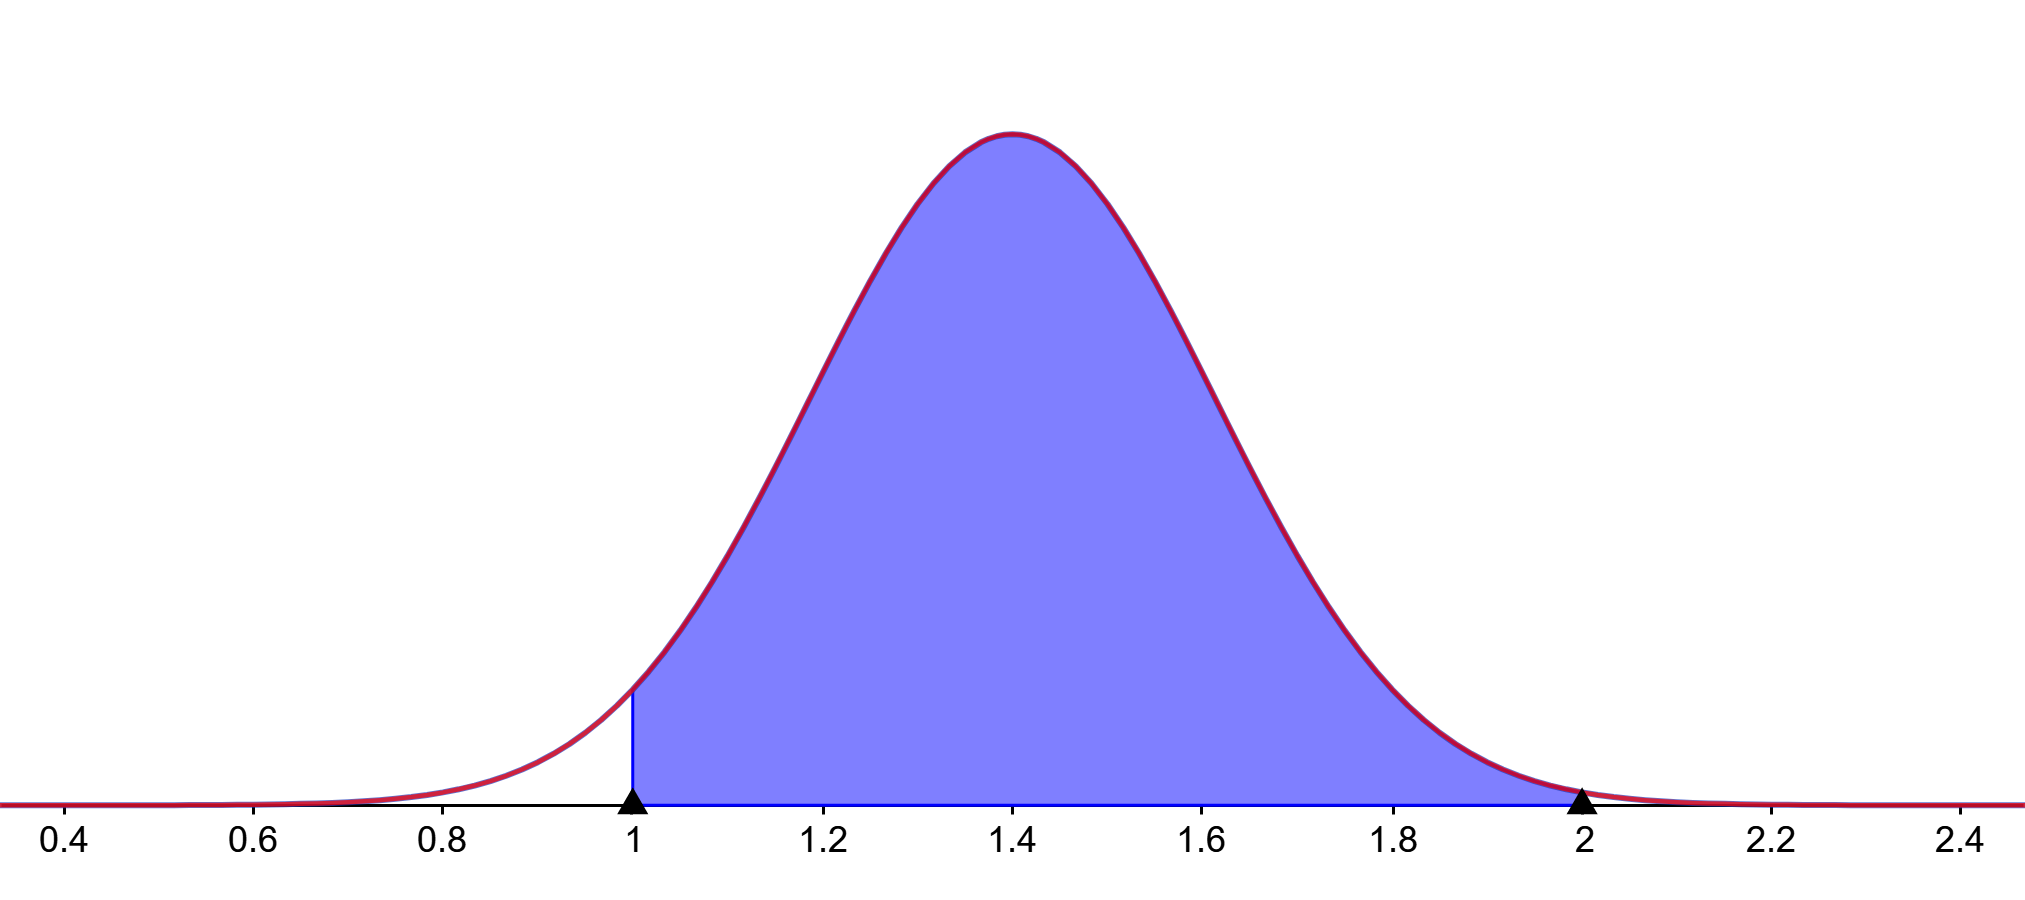
\includegraphics[scale=0.12]{geogebra-export} 
\end{center}

\section{Problema 6}
Una empresa comercializadora de café sabe que el consumo mensual (en Kg) de café por casa esta normalmente distribuida con una media desconocida $\mu$ y una desviación estándar de 0.30. Si se toma una muestra aleatoria de 36 casas y se registra su consumo de café durante un mes, ¿cual es la probabilidad de que la media de la muestra este entre los valores $\mu-0.1$ y $\mu+0.1$?.

\begin{center}
	\textbf{\textit{\textcolor{blue}{Solución:}}}\\
\end{center}

$\sigma = 0.30, \mu = ?$ y $n = 36$\\ \\
$P(\mu - 0.1 \leq \bar{X} \leq \mu + 0.1) = P(-0.1/(0.30/6) \leq Z \leq 0.1/(0.30/6))$\\
$\hspace*{4.85cm}= P(-2 \leq Z \leq 2) = P(Z \leq 2) - P(Z \leq -2)$\\
$\hspace*{4.85cm}= 0.97725 - 0.02275 = \colorbox{yellow}{$0.9545$} $


\section{Problema 7}
La distribución de las notas del examen final de Mat.I resulto ser normal $N(\mu,\sigma^2)$, con cuartiles 1 y 3 iguales a 6.99 y 11.01 respectivamente.\\
\textbf{a)} Determine la media y la varianza de la distribución de las notas.\\
\textbf{b)} Halle el intervalo $[a,b]$ centrado en $\mu$ tal que $P[a\leq \bar{X} \leq b]=0.9544$ donde $\bar{X}$ es la medida de la muestra $X_{1},X_{2},X_{3},X_{4}$ escogida de esta población.

\begin{center}
	\textbf{\textit{\textcolor{blue}{Solución:}}}\\
\end{center}

{a)\\
\begin{center}
	$Q_{1}=6.99=P_{25}$\\ 
\end{center}
\begin{center}
	$Q_{3}=11.01=P_{75}$\\
\end{center}
\begin{center}
	$Q_{2}=\frac{Q_{1}+Q_{3}}{2}=9$\\
\end{center}
\begin{center}
\colorbox{yellow}{$\mu_{\overline{x}}=9$}\\
\end{center}
\begin{center}
$P(\overline{X}\leq6.99)=0.25$\\
\end{center}
\begin{center}
$P(Z\leq \frac{6.99-9}{\sigma})=0.25$\\
\end{center}
\begin{center}
$Z = -0.68 = \frac{6.99-9}{\sigma}$\\
\end{center}
\begin{center}
\colorbox{yellow}{$\sigma = 3$}\\
\end{center}
\newpage
b)\\
\begin{center}
$P(a\leq b) = 0.9544$\\
\end{center}
\begin{center}
$P(\overline{X}\leq b) - P(\overline{X} \leq a) = 0.9544$\\
\end{center}
\begin{center}
$P(Z \leq \frac{b - \mu}{\frac{\sigma}{\sqrt{n}}})-P(Z \leq \frac{a - \mu}{\frac{\sigma}{\sqrt{n}}})=0.9544$\\
\end{center}
\begin{center}
$P(Z \leq \frac{b - \mu}{\frac{\sigma}{\sqrt{n}}})-(1-P(Z \leq \frac{b - \mu}{\frac{\sigma}{\sqrt{n}}})=0.9544$\\
\end{center}
\begin{center}
$2P(Z \leq \frac{b - \mu}{\frac{\sigma}{\sqrt{n}}})-1=0.9544$\\
\end{center}
\begin{center}
$P(Z \leq \frac{b - \mu}{\frac{\sigma}{\sqrt{n}}})=\frac{1.9544}{2}$\\
\end{center}
\begin{center}
$P(Z \leq \frac{b - \mu}{\frac{\sigma}{\sqrt{n}}})=0.9772$\\
\end{center}
\begin{center}
$Z=2=\frac{b-\mu}{\frac{\sigma}{\sqrt{n}}}=\frac{b-9}{\frac{3}{2}}$\\
\end{center}
\begin{center}
donde, \colorbox{yellow}{$b = 12$}\\
\end{center}
\begin{center}
$\frac{a-9}{\frac{3}{2}}=-2$\\
\end{center}
\begin{center}
\colorbox{yellow}{$a = 6$}
\end{center}


\section{Problema 8}
La vida útil (en miles de horas) de una batería es una variable aleatoria $X$ con función de densidad:
\begin{equation*}
f(x)= \left\{ \begin{array}{lcc}
			 2-2x &    &0\leq x \leq 1 \\
			 \\0 &       &en el resto \\
			 \end{array}
	\right.
\end{equation*}
Si $\bar{X}_{36}$ es la media de la muestra aleatoria $X_{1},X_{2}...X_{36}$  escogida de $X$, ¿con que probabilidad $\bar{X}_{36}$ es mayor que 420 horas?.

\begin{center}
	\textbf{\textit{\textcolor{blue}{Solución:}}}\\
\end{center}

X : vida util(1000hrs)\\

f(x) = 2-2x; 0 $\leq$ x $\leq$ 1\\
$\displaystyle\int_{0}^{1}f(x)=1\\
\displaystyle\int_{0}^{1}(2-2x)dx=1\\
\left2x-x^2|_0^1=2-1=1$\\
$E(x)=\mu$ \\
var(x)=$\sigma^2$\\
$P(X_{36 \succ 420 hrs})$
$P(X_{36 \succ 0.42})$\\
$\mu = E(x) = \displaystyle\int_{0}^{1}x(2-2x)dx=1$\\
$ x^2 - \frac{2x^3}{3}|_{0}^{1}=1-\frac{2}{3}=\frac{1}{3}=0.33$\\
donde, $\mu $= 0.33\\
$E(x^2) = \displaystyle\int_{0}^{1}x^2(2-2x)dx=1$\\ 
\left $\frac{2x^3}{3}$ - $\frac{x^4}{2}|_0^1$= $\frac{2}{3}$-$\frac{1}{2}$=$\frac{1}{3}=0.56$\\
\\$\sigma^2$=0.56			

$P\left(\frac{\overline{X}_{36}-\mu}{\frac{\sigma}{\sqrt{n}}}\succ \frac{0.42-0.33}{\frac{\sqrt{\frac{1}{18}}}{\sqrt{36}}}\right)$ \\
$P(Z \succ a) = 1 - P(Z \leq a)$\\
$= 1 - P(Z \leq 2.21)$\\
= 1 - 0.98645\\
\colorbox{yellow}{$= 0.0136$}

\section{Problema 9}
Sea $\bar{X}_{40}$ la media de la muestra aleatoria $X_{1},X_{2}...X_{40}$ de tamaño $n=40$ escogida de una población $X$ cuya distribución es geométrica con función de probabilidad. 
\begin{equation*}
f(x)=\frac{1}{5}\left(\frac{4}{5} \right)^{x-1},x=1,2...	
\end{equation*}
Halle la probabilidad de que la media muestral difiera de la media poblacional en a lo más el 10\% del valor de la varianza de la poblacion.

\begin{center}
	\textbf{\textit{\textcolor{blue}{Solución:}}}\\
\end{center}

\textmd{Viendo que:} \\ 
$f(x)=\dfrac{1}{5}\left(\dfrac{4}{5} \right)^{x-1}$\\
\\
$E(x) = \sum_{x=1}^{40}x f(x)$\\
$E(x)=\mu=4.99$\\
\\
$\sigma^{2}=\sum_{x=1}^{40}x^{2} f(x)-(E(x))^{2}$\\
$\sigma^{2}=44.73-4.99^{2}$\\
$\sigma^{2}=19.83$\\
$\sigma=4.45$
\\
\textmd{Teniendo ya la varianza muestral calcularemos la probabilidad:}\\
$P\left(\dfrac{\bar{x}-\mu}{\dfrac{\sigma}{\sqrt{n}}}\leq \dfrac{0.10\sigma^{2}}{\dfrac{\sigma}{\sqrt{40}}}\right) $\\
\\
$P(Z\leq (0.10)(\sqrt{40})\sigma)$\\
\\
$P(Z\leq (0.10)(\sqrt{40})(4.45))$\\
\\
$P(Z\leq 2.81)$\\
\\
$=0.99$\\
\\
\text{Rpta: La probabilidad de dicha pregunta es: \colorbox{yellow}{0.99} }


\section{Problema 10}
%%\documentclass[12pt,a4paper]{report}
\documentclass[DIV=calc,paper=a4,fontsize=11pt,openany]{book}
\usepackage[utf8]{inputenc}
\usepackage[spanish]{babel}
\renewcommand{\baselinestretch}{1.3}
\usepackage[autostyle,spanish=mexican]{csquotes}
\MakeOuterQuote{"}
\usepackage{amsmath,amsfonts,amsthm,amssymb,wasysym}
\usepackage{graphicx}
\usepackage{amsmath}
\usepackage{amsfonts}
\usepackage{latexsym}
\usepackage{enumerate}
\usepackage{amssymb}
\usepackage{makeidx}
\usepackage{tikz}
\usepackage{pstricks} 
\usepackage{cancel}
\usepackage{caption}
\usepackage{float} %flotador de label
\usepackage{wrapfig} %Permite figuras o tablas que tienen texto
\usepackage{shadow}
\usepackage{fancyhdr} %definir pie de pagina y encabesados
\usepackage{multicol}
\usepackage[all]{xy}
\usepackage{underoverlap}
\usepackage{asymptote}
\usepackage{environ}
\usepackage{multicol}
\usepgflibrary{shapes.misc}
\usepackage{MnSymbol}
\usepackage{mathrsfs}
\usepackage[left=3cm,right=3.7cm,top=2.8cm,bottom=2.7cm]{geometry}
\usepackage{pdfpages}
\usepackage[colorinlistoftodos, textwidth=3cm, shadow]{todonotes}
 \definecolor{verdeoscuro}{RGB}{6,18,97}
 
%%%encabezado y pie de pagina1
\renewcommand{\footrulewidth}{2pt}  %regla de pie de pagina
\pagestyle{fancy} %para que aparescaa regla orizontal
\columnseprule=1.2pt %regla de columna
\columnsep=25pt  %espacio en blando de la columna y texto
%encabezado

\lhead[{\vspace*{-0.2cm}\red ESTADISTICA II} ] {\bf\red UNIVERSIDAD NACIONAL DE SAN CRISTÓBAL DE HUAMANGA\ -\ ING. DE SISTEMAS }
\chead[]{}
\rhead[\rightmark]{\bf \blue }

%pie de pagina
\definecolor{blue(pigment)}{RGB}{20,70,60}
\lfoot[]{\bf }
\cfoot[]{}
\rfoot[]{\vspace*{-0.8cm}\fcolorbox{black}{white}{\Large\bfseries\color{blue(pigment)} {\thepage}}}
\usetikzlibrary{shadows}                          
\newcommand{\preg}[1]{
   \par\vspace{0.6em}\noindent 
                           
\begin{tikzpicture}[baseline=(X.base)]\node       
	[drop shadow,fill=black,draw,very thin] (X) {\color{white} \textsf{\textbf{#1}}}; 
\end{tikzpicture}\hspace{0.4cm}}
 
%sombra%                         
\newcommand{\sombra}[1]{                          
\begin{tikzpicture}[baseline=(X.base)]\node       
	[drop shadow,fill=white,draw,very thin] (X) {#1}; 
\end{tikzpicture}}

%ejercicios%
\newcommand{\Ejercicio}[1]{   
\begin{tikzpicture}
	\node[rounded rectangle, white, fill=black!70, draw]
	{\sf {Ejercicio} {\normalsize  #1}};
\end{tikzpicture}
}
\renewcommand{\thesection}{\arabic{section}}
%%%%%%%contador%%%%%%%%
\newcounter{contador}[section] 
\setcounter{contador}{0}       

%%%%%%%%definimos ambiente pregunta y solucion%%%%%%%%%%%%
\usepackage{colortbl}                                                                               
\definecolor{col}{RGB}{45,07,107}

%solucion%                    
\newcommand\sol{\noindent                                         
 \\[0.4em]
  { \slshape \color{red}\textbf{Resolución}}
  \\[0.3em]\noindent  }
                     
\makeatother
                                
%%%%comandos particulares%%%%
\newcommand{\af}{\alpha}
\newcommand{\D}{\pmb{D}}
\newcommand{\be}{\beta}
\newcommand{\te}{\theta}
\newcommand{\al}{\displaystyle}
\newcommand{\med}{\scriptstyle}
\newcommand{\imp}{\Rightarrow}
\newcommand{\impp}{\Longleftrightarrow}
\newcommand{\im}{\rightarrow}
\newcommand{\p}{\cdot}
\newcommand{\ca}{\cancel}
\newcommand{\tri}{\therefore}
\newcommand{\sen}{\mathop{\rm sen}\nolimits}
\newcommand{\tg}{\mathop{\rm tg}\nolimits}\newcommand{\ct}{\mathop{\rm ctg}\nolimits}
\newcommand{\R}{\mathbb{R}}
\newcommand{\Z}{\mathbb{Z}}
\newcommand{\N}{\mathbb{N}}
\newcommand{\se}{\overline}
\newcommand{\ang}{\measuredangle}
\newcommand{\an}{\angle}
\newcommand{\tr}{\triangle}
\newcommand{\g}{^\circ}
\newcommand{\spa}{\smallskip}
\newcommand{\spac}{\medskip}
\newcommand{\brazo}{\underbrace}
\newcommand{\medi}{\mbox{m}\measuredangle}
\newcommand{\f}{\frac}
\newcommand{\dist}{\vspace{-0.5cm}}
\newcommand{\rad}{\;\mbox{rad}}\newcommand{\bi}{\bullet\;\;}
\newcommand{\Del}[1]{\left[#1\right]}
\newcommand{\del}[1]{\left(#1\right)}
\newcommand{\sect}[1]{\leftslice\scriptscriptstyle{#1}}
\newcommand{\q}{\sqrt}
\newcommand{\y}{\;\wedge\;}
\newcommand{\oo}{\;\vee \;}
\newcommand{\sii}{\;\Leftrightarrow\;}
\newcommand{\pt}{\times}
\newcommand{\s}{\sec\mathsf{h}}
\newcommand{\ta }{\tan\mathsf{h}}
\newcommand{\limt}{\lim_{n\rightarrow \infty}}
\newcommand{\prt}{\partial}
\newcommand{\M}{\geq}
\newcommand{\m}{\leq}
\newcommand{\vol}{\mathrm{Vol}}
\newcommand{\area}{\mathrm{Area}}
\newcommand{\yy}{\overline{y}}
\newcommand{\vx}{\overline{x}}
\newcommand{\hs}{\hspace{0.6cm}}
\newcommand{\dd}{\mathrm{d}}
\newcommand{\n}{\nabla}
\usepackage{amsmath}
\usepackage{graphicx,tcolorbox}
\definecolor{blue(pigment)}{RGB}{20,70,60}
\definecolor{som}{RGB}{68,05,5}
\usetikzlibrary{shadows} 

%---------RTA----------%
\newcommand{\ptas}[1]{
\begin{flushright}
	\begin{tikzpicture}
	\node[rounded rectangle, white, fill=black!70, draw]
	{\sf {clave} {\normalsize #1}};
	\end{tikzpicture}
\end{flushright}}
% Estilos: Sonny, Lenny, Glenn, Conny, Rejne, Bjarne, Bjornstrup
\usepackage[Sonny]{fncychap}


\begin{document}%INICIO DEL DOCUMENTO 


\Ejercicio{10}\\

El tiempo de vida de una bateria es una variable aleatoria \textit{X} con distribución exponencial de parámetro: $1/\theta$. Se escoge una muestra de n baterías\\
a) Halle el error estandar de la media muestral $\overline{X}$\\
b) Si la muestra aleatoria es de tamaño $ n = 64 $, ¿con que probabilidad diferirá $\overline{X}$ del verdadero valor $\theta$ en menos de un error estándar?\\
c) ¿Qué tamaño de muestra mínimo sería necesario para que la media muestral $\overline{X}$ tenga un error estándar menor a un $5\%$ del valor real de $\theta?$\\
d) Asumiendo muestra grande, ¿qué tamaño de muestra sería necesario para que $\overline{X}$ difiera de $\theta$ en menos de $10\%$
de $\theta$ con $95\%$ de probabilidad?\\

\textbf{\textit{\textcolor{blue}{Solución:}}}\\

a) 
\begin{center}
$f(x) = \dfrac{1}{\theta}e^{\frac{-x}{\theta}}$ ; $x\geqslant 0$
\end{center}
\begin{center}
$\sqrt{Var(\overline{X})} = \dfrac{\theta}{\sqrt{n}}$ \  error estandar
\end{center}
\begin{center}
$Var(\overline{X}) = \dfrac{\theta^{2}}{n}$
\end{center}
\[ E(x) = u = \int_{0}^{+\infty} \! \dfrac{x}{e}e^\frac{-x}{\theta} \, dx 
\]
\[\gamma(\alpha)=\int_{0}^{+\infty} \! y^{\alpha-1}e^{-y} \, dy\]
\begin{center}
$(\alpha-1)!$ \ ; $ \alpha \in N $
\end{center}
\begin{center}
$\gamma(\alpha) = (\alpha-1)!\gamma(\alpha-1)$ ; para $\alpha \neq N$
\end{center}
\[ E(x) = u = \theta\int_{0}^{+\infty} \! (\dfrac{x}{\theta})^{2-1}e^\frac{-x}{\theta} \, d(\frac{x}{\theta})
\]
\begin{center}
$\gamma(2)=(2-1)! = 1$
\end{center}
\begin{center}
$ E(x)= \theta $
\end{center}
\[ E(x^{2})  \theta^{2}\int_{0}^{+\infty} \! (\dfrac{x}{\theta})^{3-1}e^\frac{-x}{\theta} \, d(\frac{x}{\theta})
\]
\begin{center}
$E(x^{2})=2\theta^{2}$
\end{center}
\begin{center}
$\gamma(3)= 2!= 2$
\end{center}
\begin{center}
\colorbox{yellow}{$\sigma^{2} = Var(x) = 2\theta^{2}-\theta^{2} = \theta^{2}$}
\end{center}
\newpage
b) Teorema Central de Limite\\
\begin{center}
\includegraphics[scale=0.15]{Imagenes/geogebra-export.png} 
\end{center}
\begin{center}
$P(\mid\overline{X}- \sigma \mid \leq \dfrac{\theta}{\sqrt{n}} \cong 0.68$
\end{center}
\begin{center}
$P(-\theta \leq x-4\leq \theta)$
\end{center}
\begin{center}
$P(\mid x - u \mid \leq 2\theta) \cong 0.9544$
\end{center}
\begin{center}
$P(\mid x - u \mid \leq 3\theta) \cong 0.99$
\end{center}
\begin{center}
$u\overline{X} = u = \theta$
\end{center}
\begin{center}
$Var(\overline{X}) = \theta^{2}x = \theta^{2}$
\end{center}
\begin{center}
$  P(\mid \overline{X} - \theta \mid \leq \dfrac{\theta}{\sqrt{n}})$
\end{center}

\begin{center}
$P( \overline{X} - \theta  \leq \dfrac{\theta}{8}) = P\left( \dfrac{\overline{X}- \theta}{\frac{\theta}{8}} \leq \dfrac{\frac{\theta}{8}}{\frac{\theta}{8}}\right)$ 
\end{center}
\begin{center}
$ P( \overline{X} - \theta  \leq \dfrac{\theta}{8}) = P(z \leq 1$
\end{center}
\begin{center}
\colorbox{yellow}{$P( \overline{X} - \theta  \leq \dfrac{\theta}{8}) = 0,68$} 
\end{center}
c)
\begin{center}
$\dfrac{\theta}{\sqrt{n}} < 0.050\theta \Rightarrow \dfrac{1}{\sqrt{n} < 0,05}$
\end{center}
\begin{center}
$1\dfrac{1}{0.05}<\sqrt{n} \Rightarrow 20^{2} < \sqrt{n}^{2}$
\end{center}
\begin{center}
\colorbox{yellow}{$20 < \sqrt{n} \Rightarrow 400 < n$}
\end{center}
d)
\begin{center}
$P(\mid \overline{X}-u \mid < 0.1\theta)=0.95$
\end{center}
\begin{center}
$P\left( \dfrac{\overline{X}-u}{\frac{\sigma}{\sqrt{n}}} < \dfrac{0.1\theta}{\frac{\sigma}{\sqrt{n}}}\right)= 0.95$
\end{center}
\begin{center}
$P(\mid Z \mid < 0.1\sqrt{n}) = 0.95$
\end{center}
\begin{center}
$P(-0.1\sqrt{n} < z < 0.1\sqrt{n}) = 0.95$
\end{center}
\begin{center}
$P(z < 0.1\sqrt{n})- (1-P(z < 0.1\sqrt{n}) = 0.95$
\end{center}
\begin{center}
$2P( z < 0.1\sqrt{n}) = 1.95$
\end{center}
\begin{center}
$P(z < 0.1\sqrt{n}) = 0.975$
\end{center}
\begin{center}
$0.1\sqrt{n} = 1.96$
\end{center}
\begin{center}
$\sqrt{n} = 19.6$
\end{center}
\begin{center}
\colorbox{yellow}{$n = 385 $}
\end{center}











\end{document}%FINAL DEL DOCUMENTO%

El tiempo de vida de una bateria es una variable aleatoria \textit{X} con distribución exponencial de parámetro: $1/\theta$. Se escoge una muestra de n baterías\\
a) Halle el error estandar de la media muestral $\overline{X}$\\
b) Si la muestra aleatoria es de tamaño $ n = 64 $, ¿con que probabilidad diferirá $\overline{X}$ del verdadero valor $\theta$ en menos de un error estándar?\\
c) ¿Qué tamaño de muestra mínimo sería necesario para que la media muestral $\overline{X}$ tenga un error estándar menor a un $5\%$ del valor real de $\theta?$\\
d) Asumiendo muestra grande, ¿qué tamaño de muestra sería necesario para que $\overline{X}$ difiera de $\theta$ en menos de $10\%$
de $\theta$ con $95\%$ de probabilidad?\\

\begin{center}
\textbf{\textit{\textcolor{blue}{Solución:}}}\\
\end{center}

a) 
\begin{center}
	$f(x) = \dfrac{1}{\theta}e^{\frac{-x}{\theta}}$ ; $x\geqslant 0$
\end{center}
\begin{center}
	$\sqrt{Var(\overline{X})} = \dfrac{\theta}{\sqrt{n}}$ \  error estandar
\end{center}
\begin{center}
	$Var(\overline{X}) = \dfrac{\theta^{2}}{n}$
\end{center}
\[ E(x) = u = \int_{0}^{+\infty} \! \dfrac{x}{e}e^\frac{-x}{\theta} \, dx 
\]
\[\gamma(\alpha)=\int_{0}^{+\infty} \! y^{\alpha-1}e^{-y} \, dy\]
\begin{center}
	$(\alpha-1)!$ \ ; $ \alpha \in N $
\end{center}
\begin{center}
	$\gamma(\alpha) = (\alpha-1)!\gamma(\alpha-1)$ ; para $\alpha \neq N$
\end{center}
\[ E(x) = u = \theta\int_{0}^{+\infty} \! (\dfrac{x}{\theta})^{2-1}e^\frac{-x}{\theta} \, d(\frac{x}{\theta})
\]
\begin{center}
	$\gamma(2)=(2-1)! = 1$
\end{center}
\begin{center}
	$ E(x)= \theta $
\end{center}
\[ E(x^{2})  \theta^{2}\int_{0}^{+\infty} \! (\dfrac{x}{\theta})^{3-1}e^\frac{-x}{\theta} \, d(\frac{x}{\theta})
\]
\begin{center}
	$E(x^{2})=2\theta^{2}$
\end{center}
\begin{center}
	$\gamma(3)= 2!= 2$
\end{center}
\begin{center}
	\colorbox{yellow}{$\sigma^{2} = Var(x) = 2\theta^{2}-\theta^{2} = \theta^{2}$}
\end{center}

b) Teorema Central de Limite\\
\begin{center}
	\includegraphics[scale=0.15]{ANDERSON/Imagenes/geogebra-export} 
\end{center}

\begin{center}
	$P(\mid\overline{X}- \sigma \mid \leq \dfrac{\theta}{\sqrt{n}} \cong 0.68$
\end{center}
\begin{center}
	$P(-\theta \leq x-4\leq \theta)$
\end{center}
\begin{center}
	$P(\mid x - u \mid \leq 2\theta) \cong 0.9544$
\end{center}
\begin{center}
	$P(\mid x - u \mid \leq 3\theta) \cong 0.99$
\end{center}
\begin{center}
	$u\overline{X} = u = \theta$
\end{center}
\begin{center}
	$Var(\overline{X}) = \theta^{2}x = \theta^{2}$
\end{center}
\begin{center}
	$  P(\mid \overline{X} - \theta \mid \leq \dfrac{\theta}{\sqrt{n}})$
\end{center}

\begin{center}
	$P( \overline{X} - \theta  \leq \dfrac{\theta}{8}) = P\left( \dfrac{\overline{X}- \theta}{\frac{\theta}{8}} \leq \dfrac{\frac{\theta}{8}}{\frac{\theta}{8}}\right)$ 
\end{center}
\begin{center}
	$ P( \overline{X} - \theta  \leq \dfrac{\theta}{8}) = P(z \leq 1$
\end{center}
\begin{center}
	\colorbox{yellow}{$P( \overline{X} - \theta  \leq \dfrac{\theta}{8}) = 0,68$} 
\end{center}
c)
\begin{center}
	$\dfrac{\theta}{\sqrt{n}} < 0.050\theta \Rightarrow \dfrac{1}{\sqrt{n} < 0,05}$
\end{center}
\begin{center}
	$1\dfrac{1}{0.05}<\sqrt{n} \Rightarrow 20^{2} < \sqrt{n}^{2}$
\end{center}
\begin{center}
	\colorbox{yellow}{$20 < \sqrt{n} \Rightarrow 400 < n$}
\end{center}
d)
\begin{center}
	$P(\mid \overline{X}-u \mid < 0.1\theta)=0.95$
\end{center}
\begin{center}
	$P\left( \dfrac{\overline{X}-u}{\frac{\sigma}{\sqrt{n}}} < \dfrac{0.1\theta}{\frac{\sigma}{\sqrt{n}}}\right)= 0.95$
\end{center}
\begin{center}
	$P(\mid Z \mid < 0.1\sqrt{n}) = 0.95$
\end{center}
\begin{center}
	$P(-0.1\sqrt{n} < z < 0.1\sqrt{n}) = 0.95$
\end{center}
\begin{center}
	$P(z < 0.1\sqrt{n})- (1-P(z < 0.1\sqrt{n}) = 0.95$
\end{center}
\begin{center}
	$2P( z < 0.1\sqrt{n}) = 1.95$
\end{center}
\begin{center}
	$P(z < 0.1\sqrt{n}) = 0.975$
\end{center}
\begin{center}
	$0.1\sqrt{n} = 1.96$
\end{center}
\begin{center}
	$\sqrt{n} = 19.6$
\end{center}
\begin{center}
	\colorbox{yellow}{$n = 385 $}
\end{center}


\newpage

\section{Problema 11}
La utilidad por la venta de cierto articulo, en miles de soles, es una variable aleatoria con distribución normal. En el 5\% de las ventas de utilidad ha sido menos de 3.42, mientras que el 1\% de las ventas ha sido mayor que 19,32. Si se realizan 16 operaciones de ventas,¿cual es la probabilidad de que el promedio de la utilidad por cada operación?

\begin{center}
	\textbf{\textit{\textcolor{blue}{Solución:}}}\\
\end{center}

	\textmd{Teniendo en cuenta:} \\ 
$P(x \leq 3.42)= 0.05$ \\
$P(x \geq 19.32) = 0.01 \equiv P(x \leq 19.32) = 0.99$ \\
\textmd{Con $n = 16$ y  $\mu$,$\sigma$ desconocidas}\\
$P(x \leq 3.42)= 0.05 \Rightarrow P(Z \leq \frac{3.42 -\mu}{\sigma} )= 0.05 \Rightarrow \frac{3.42 -\mu}{\sigma} = -1.64 \Rightarrow \sigma = \frac{3.42 -\mu}{-1.64} $ \\ \\
$P(x \geq 19.32)= 0.01 \Rightarrow P(Z \leq \frac{19.32 -\mu}{\sigma} )= 0.99 \Rightarrow \frac{19.32 -\mu}{\sigma} = 2.33 \Rightarrow \sigma = \frac{19.32 -\mu}{2.33}$\\ \\
\textmd{Igualando ambos sigmas obtenemos: $\frac{3.42 -\mu}{-1.64}=\frac{3.42 -\mu}{2.33}  \Rightarrow \mu = 10.01$ y reemplazandolo se obtiene que: $\sigma =4  $; luego:}\\
$P(10 \leq x \leq 12)\Rightarrow P(x \leq 12) - P(x \leq 10)\Rightarrow P(Z \leq \frac{12-10.01}{\frac{3.99}{4}}) - P(Z \leq \frac{10-10.01}{\frac{3.99}{4}}) \\ \\ \Rightarrow P(Z \leq 1.99) - P(Z \leq 0.01)\Rightarrow P(Z \leq 1.99) - 1 + P(Z \leq 0.01) \Rightarrow 0.97 - 1 + 0.5 = 0.47$

\section{Problema 12}
La vida útil de cierta marca de llantas radiales es una variable aleatoria $X$ cuya distribución es normal con $\mu=38,000 Km$. y $\sigma=3,000 Km$.\\
\textbf{a)} Si la utilidad $Y$ (en \$) que produce cada llanta está dada por la relación:\\
$Y=0.2X+100$, ¿cual es la probabilidad de que la utilidad sea mayor que 8,900\$?\\
\textbf{b)} Determine el numero de tales llantas que debe adquirir una empresa de transporte para conseguir una utilidad media de al menos 7541\$ con probabilidad 0.996.

\begin{center}
	\textbf{\textit{\textcolor{blue}{Solución:}}}\\
\end{center}

\vspace{0.5em}
$Y = 0.2X + 100 \Rrightarrow E[Y] = 0.2E[X] + 100 = 0.2(38000) + 100 = 7700$\\\vspace{0.5em}
$Y = 0.2X + 100 \Rrightarrow Var[Y] = 0.2Var[X] + 100 = 0.0.4 (9000)^{2} + 0 = 360000 $ \\\vspace{0.5em}
$Y \rightarrow X(7700,360000)$\\

\textbf{a)}\\

$P(Y > 8900) \Rrightarrow 1-P(Y \leq 8900)\\ \Rrightarrow 1-P(Z \leq \frac{8900 - 7700}{\sqrt{360000}/\sqrt{1}}) \Rrightarrow 1 - P(Z \leq \frac{1200}{600}) \Rrightarrow 1 - P(Z \leq 2) \Rrightarrow 1 - 0.97725 = 0.02275$\\

\textbf{b)}\\

$P(Y > 7541) = 0.996 \Rrightarrow 1-P(Y \leq 7541) = 0.996\\ \Rrightarrow P(Z \leq \frac{7541 - 7700}{\sqrt{360000}/\sqrt{n}}) = 1 - 0.996 \Rrightarrow P(Z \leq \frac{-154(\sqrt{n})}{600}) = 0.004\\
\Rrightarrow \frac{-154(\sqrt{n})}{600} = -2.65 \Rrightarrow \sqrt{n} = \frac{(600)(2.65)}{159} \Rrightarrow \ sqrt{n} = 10 \Rrightarrow n = 100$


\section{Problema 13}
Un proceso automático llena bolsas de café cuyo peso neto tiene una media de 250 gramos y una desviación estándar de 3 gramos. Para controlar el proceso, cada hora se pesan 36 bolsas escogidas al azar; si el peso neto medio esta entre 249 y 251 gramos se continua con el proceso aceptando que el peso neto medio es 250 gramos y en caso contrario, se detiene el proceso para reajustar la maquina.\\
\textbf{a)} ¿Cuál es la probabilidad de detener el proceso cuando el peso neto medio realmente es 250 gramos?.\\
\textbf{b)} ¿Cuál es la probabilidad de aceptar que el peso neto promedio es 250 cuando realmente es de 248 gramos?.\\

\begin{center}
	\textbf{\textit{\textcolor{blue}{Solución:}}}\\
\end{center}

\textbf{a)}  desarrollamos la probabilidad para peso neto de 250 gramos.\\

\begin{center}
$N(50,3) P(249 \leq \bar{X} \leq 251) n=36$
\end{center}
\begin{center}
	$P(249 \leq \bar{X} \leq 251)$
\end{center}

\begin{center}
	$P(\bar{X} \leq 249)+1-P(\bar{X} \leq 251)$
\end{center}
\begin{center}
	$P\left(Z \leq \frac{249-250}{\frac{3}{\sqrt{36}}}\right) +1-P\left(Z \leq \frac{251-250}{\frac{3}{\sqrt{36}}}\right)$
\end{center}

\begin{center}
	$P(Z \leq -2)+1-P(Z \leq 2)$
\end{center}

\begin{center}
	$0.02273+1-0.97725$
\end{center}
\begin{center}
	$=\colorbox{yellow}{$0,0456$}$
\end{center}

\textbf{b)} 

\begin{center}
	$P(249 \leq \bar{X} \leq 251)$
\end{center}
\begin{center}
	$P\left (Z \leq \frac{249-250}{\frac{3}{\sqrt{36}}}\right)$
\end{center}
\begin{center}
	$P(Z \leq -2)$
\end{center}
\begin{center}
	$=\colorbox{yellow}{$0.02275$}$
\end{center}


\end{document}